\section{Introduction}
In the past decade, with the introduction of technology that can store huge amounts of data, a large amount of musical data is increasingly available to public on different application platforms such as Spotify. As the number of musical data in our phones and Internet keeps increasing, there is a need to characterize each music track so that finding a specific song in a large archive of music would not be a problem. Musical genres are commonly used to describe and characterize songs for music information retrieval. Pachet suggests that genre of music can be the best general information for music content description \cite{Pachet:2003}. Hence, a system that can classify musical genres can solve the problem of locating a specific sound track on any device. 

The only problem with musical genre classification is the fact that the definition of genre is very subjective by its nature and there exists thousands of genres or sub-genres. It is also important to note that, the definition of music genre tends to change with time, as what we call Rock song today is very different from the rock songs twenty years ago. Even though musical genres are subjective, there are certain features that can easily distinguish between different genres. By using features such as distribution of frequency or the number of beats, it is possible to classify main genres of music. For classification of musical genres, various approaches have been proposed. Unfortunately, most of these approaches have been proven to show accuracy around 60-70\%. Therefore, new approaches that can maximize classification accuracy must be considered.  

Hence, we try to improve the classification accuracy of music genre classification of audio signals in this work. Specifically, we use a wide range of machine learning algorithms, including k-Nearest Neighbor (k-NN) \cite{KNN:2009}, k-Means Clustering \cite{Clustering:2001}, Support Vector Machines \cite{SVM:2006}, Gaussian Mixture Models \cite{Pachet:2003} and different types of Neural Networks to classify the following 5 genres: metal, classical, blues, pop, country. 

Our main goal in this study is to maximize the classification accuracy of 5 genres and compare different methods of machine learning for classification of audio signals. We use state-of-the-art machine learning platforms such as PyTorch \cite{PyTorch:2017} to introduce deep learning into our project. We experiment with different neural network architectures and types of neural network. Moreover, we use Mel Frequency Cepstral Coefficients (MFCC) \cite{MFCC:2011} to extract useful information from musical data as recommended by past work in this field.
To summarize, we make three main contributions in this paper:
\begin{itemize}
  \item We experiment with a wide range of machine learning algorithms and state their classification accuracy for 5 different genres. 
  \item We propose a method for feature extraction and audio processing that is dependent on both MFCC and PCA. We also discuss the significance of such methods. 
  \item We report experimental data that describe the overall effectiveness of our classification methods by including confusion matrices. 
\end{itemize}

----->>> ADD a paragraph that states experimental results briefly!!!! <<<-------- 

\section{Related Work}\label{sec:related}

The development of music genre classification has been increasing rapidly in the past decade. Many approaches have been proposed that build different models for genre classification. Some approaches concentrate on the processing of audio signals, whereas some approaches try to combine audio signals with lyrics from each musical track to increase accuracy. Some of the related work to our project is presented below. 

Firstly, Tzanetakis and Cook \cite{GTZAN:2002} introduced different feautres to organize musical tracks into a genre by using k-NN and Gaussian Mixture Model (GMM) methods. Three different feature sets for speaking to tumbrel surface, rythmic substance and pitch substance of music signse were suggested. They also introduced a dataset for music genre classification (GTZAN Dataset \cite{GTZAN:2002}), which is widely used today in many project, including ours. 

Furthermore, Aucouturier and Pachet \cite{Pachet:2003} used GMM and utilized Monte Carlo procedures for evaluation of KL divergence, which was used in a k-NN classifier. They conveyed some significant component sets for musical information retrieval that we use in our work, specifically the MFCC. 

Apart from models such as GMM or k-NN, Feng \cite{Feng:2016} proposed an approach that uses Restricted Boltzmann machine algorithm to build deep belief neural networks. By generating more dataset from the original limited music tracks, he shows great improvement in the classification accuracy and describes the significance of neural networks for music genre classification. 

Xing et. al. \cite{Xing:2016} proposes a similar approach that uses convolutional neural networks. By combining max and average pooling to provide more more statistical information to higher neaural networks and applying residual connections, Xing et. al. \cite{Xing:2016} improves the classification accuracy on the GTZAN data set greatly. Li, Chan and Chun \cite{Chun:2010} recommend a very similar technique to concentrate musical example included in audio signals by using convolutional neural networks. They present their revelation of the perfect parameter set and best work on CNN for music genre classification.

Finally, Smaragdis and Whitman \cite{Smaragdis:2002} presents a very interesting musical style identification scheme based on simultaneous classification of auditory and textual data. They combine musical and cultural features of audio tracks for intelligent style detection. They suggest that addition of cultural attributes in feature space improves the proper classification of acoustically dissimilar music within the same style.

-->> Add a paragraph that compares our work to above <<-- 
As compared to these works,...
%%%%%%%%%%%%%%%%%%%%%%%%%%%%

\section{Proposed Approach}\label{sec:approach}
% Dataset --> Feature Extraction --> Dimensionality Reduction --> Algorithms 
\subsection{Musical Dataset}
For musical data, Marsyas is an open source software framework for Music Information Retrieval with the GTZAN Genre Collection Database, which has 10 genres and each genre has 100 30-second audio tracks. All the tracks are 22050 Hz Mono 16-bit audio files in .au format. 

For this project, we chose five distinct genres; classical, metal, blues, pop, country. Hence, our dataset was 500 songs total, from which we used 80\% for training and 20\% for testing. We chose five very distinct genres as previous works \cite{Chun:2010} suggest more than 5 genres can decrease accuracy a lot and introduces many problems. 

\subsection{Feature Extraction: Mel Frequency Cepstral Coefficients (MFCC)}
Previous works \cite{MFCC:2011} on music classification and processing of audio signals directed us to use MFCC (Mel Frequency Cepstral Coefficients) as a method for feature extraction so that time domain waveforms can be represented in the frequency domain in a mel-scale. For the process of MFCC, we first computed the spectogram of each waveform by using Fast Fourier Transform and a Hamming Window. Then, we mapped each frequency to mel scale, as mel scale is the best scale for human ears. The mel spectogram of a song from each genre is shown on Figures 1 through 5, so that the difference between each genre can be visualized. After computing the mel-spectograms of each song, we applied discrete cosine transform (DCT) and then removed the very high frequency values from our data. At the end, we had an MFCC array of each song, where we stacked all them together, created appropriate labels for each genre and constructed our training and testing datasets. As stated, we used 80\% for training and 20\% for testing our classifiers. 

% Figure 1-5 --> Mel-spectograms 

\subsection{Dimensionality Reduction with Principal Component Analysis (PCA)}
After feature extraction and construction of final dataset, we thought of using dimensionality reduction before putting out data through classifiers. Since Principal Component Analysis (PCA) is a well-known and effective method for reduction of dimensions, we used PCA on our dataset. A realistic choice for number of reduced dimensions is to visualize the data with different PCA values and then pick the minimum dimension that can keep at least 95\% of the significant components. The visualization of our data with respect to different PCA dimensions and the corresponding eigenvectors is shown on Figure 6. Note that figures 7 and 8 also present a visualization of each genre in 2 and 3 dimensions. After extensive analysis of the visualization, we reduced the dimensionality to 16. Even though 16 dimensions performed very well on classifiers such as k-NN or SVM, we had to use much bigger dimensions for our neural network, since neural networks need much more data in practice. 

% Figure 6 --> PCA vs. Eigenvecs

% Figure 7 --> 2-dimensional plt 

% Figure 8 --> 3-dimensional plt 

\subsection{Machine Learning Algorithms}
\subsubsection{\textbf{K-Nearest Neighbor (K-NN)}}
The first algorithm we used is the very famous and effective k-closest neighbors algorithm. k-NN is a non-linear algorithm that can detect direct or indirect spread of data. It is very effective for huge amounts of data. The only downside of k-NN is the fact that it makes hard decisions and might produce low classification accuracy. The most significant computation in this algorithm is measuring the distance between different points in our dataset. We used Euclidean distance for k-NN, which produced good results. After our experiments, we also found that k=5 produced the best results. 

\subsubsection{\textbf{Support Vector Machines (SVM)}}
The second technique we used is the support vector machine (SVM), which is a directed organization method that discovers the extreme boundary splitting two classes of information \cite{SVM:2006}. 

\subsubsection{\textbf{Gaussian Mixture Models (GMM)}}

\subsubsection{\textbf{K-Means Clustering}}

\subsubsection{\textbf{Simple 3-layer Neural Network}}

\subsubsection{\textbf{Convolutional Neural Network (CNN)}}

\subsubsection{\textbf{Super-Classifier (SC)}}

\section{Experimental Results}\label{sec:results}

\subsection{Experiment Setup}
The experimental setup for computation of classification accuracies were quite simple. After extracting features of our data through MFCC and applying PCA, we saved our training and testing datasets into a file, so that we do not have to do all the computations again. Then, we wrote a script that loads the training and testing datasets, and then puts the training data as an input to each of our classifiers with the corresponding genre labels. After training on each classifier, we computed predictions of each song and compared each label with its groun truth. Finally, we outputted the classification accuracy of each classifier and their confusion matrices, which are shown in Figure 9 through 16.

\subsection{Classification Accuracy}

\section{Conclusion}\label{sec:conclusion}
@@@@@@@@@@@@@@@@@@@@@@@@@@@
%\section{Future Work}\label{sec:future_work}

%%%%%%%%%%%%%%%%%%%%%%%%%
Our goal in this paper is to present and evaluate a formula to quantify instruction criticality and sort low-level instructions by their fault tolerance. This instruction criticality metric would be used to generate reliable source code and reduce the overhead in system reliability approaches applied today. 

Our proposed approach for reliable code generation takes three inputs: Original source code to be improved upon, an overhead limit for critical systems and a variable $\alpha$ that decides on the significance of SDC and Crash tolerance of the system. The main objective behind the approach is to decide on the number of instructions that can be improved based on our proposed criticality formula and then generate reliable source code. Hence, our approach outputs a very similar source code as the input but with added fault tolerance. Note that, reliability technique applied is orthogonal to our approach. We focus on where and when to apply this reliability technique. Therefore, our proposed mechanism can potentially work with any source code level reliability technique. 

In Figure \ref{fig:big_picture2}, we present a high-level description of our approach for reliable code generation and instruction criticality. After taking in the inputs, we calculate each instruction's criticality value based on their location in the program and their place on our definition of SDC and Crash metric. Finally, this criticality value is improved by taking $\alpha$ and the number of times the instruction would dynamically execute into consideration. Dynamic execution statistics are collected using profilers embedded to the compiler framework. After each instruction's criticality is calculated, we sort these instructions by their criticality and eliminate the instructions that are outside the given overhead limit. Therefore, we only apply the reliability enhancement technique to instructions within the tolerated overhead limit. While our baseline overhead limitation considers performance as a percentage, it can be extended to other types of overheads such as energy. In the next step, we apply the state-of-the-art reliability techniques on the instructions to be improved upon and then output the reliable source code. 

\begin{figure}[!t]
\begin{center}
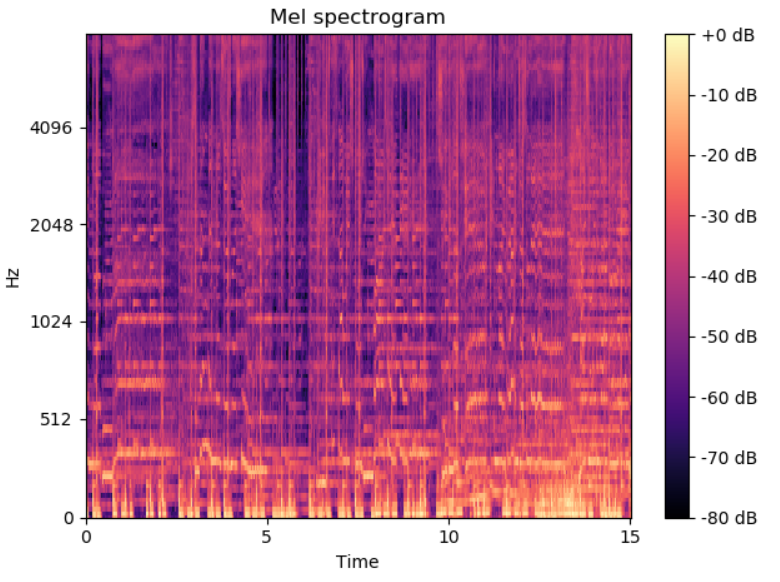
\includegraphics[scale=0.3]{./figures/pop.png}
\end{center}
\caption
{
High level sketch of our reliable source code generation approach based on instruction criticality formula. $\alpha$ is defined as a user input where it quantifies the relative importance of SDC and Crash tolerance of the original source code. The overhead limit is another user input that sets the limit for the instructions to be improved in the source code. 
}
\label{fig:big_picture2}
\end{figure}

Note that our approach may not generate a program that is fully fault-tolerant. Our goal in this work is to show that instruction criticality can actually be quantified as a value and then can be further used for reliable code generation in a selective manner. We achieve this by defining two metrics, SDC and Crash rankings, based on instruction type. These metrics are created and defined after conducting thousands of fault-injection experiments and analyzing the data. Our definition of these metrics is important for our work and affects the instruction criticality value significantly. The details of the fault-injection experiments and quantifying instruction criticality are explained in the next subsections. 


\subsection{Fault-Injection}
%Explain how we conducted experiments
%Explain different types of programs used 
%Explain pattern analysis
%Provide some data 
%Provide SDC and Crash Graphs --> Motivation 

Fault-injection experiments and their results were used to estimate a criticality value for each instruction in the source code. These experiments were conducted for each instruction in a program considering the program's Control Flow Graph (CFG). Based on the Crash and Silent Data Corruption rates in each basic block, different patterns were extracted to measure criticality based on CFG. 

The experiments were conducted using LLFI \cite{LLFI:2015}, which injects faults into the LLVM IR of the application source code. Since LLFI injects faults systematically in a reproducible manner, bit-flip injections were conducted on each instruction for at least a thousand times. Specifically, on each fault injection, a single bit is flipped on a certain instructions in a random manner. Then, for each instruction, we trace the effects of fault injection on the application code and output. We also look at the affected instructions after each injection to spot instruction types that may damage the output of the program the most. 

We used different types of programs from different application domains. From programs that perform many floating operations (Factorial) to programs that are mostly dependent on huge amounts of data (QSort), we injected faults to a wide variety of applications. To have sufficient coverage, we tested our approach on programs that had very different and specific control flows with nested if statements and for loops (Nested If/Else). We tried to analyze how a change in control flow would affect the results of a program. Hence, we were able to deduce a pattern on instruction criticality that can be applied on any application.
 
Our pattern analysis was based on the SDC and Crash rates of a program where we calculated the average fault percentage of each instruction according to its location. Based on this analysis, we observed that Silent Data Corruption (SDC) rates tend to increase if the instruction is in the later basic blocks of the program, as seen in Figure 2. We also see that crash rates increase if the instruction is located at the beginning of the program, as shown in Figure 3. Based on these observations, we conclude that location of the instruction in the control flow is a very significant aspect in the fault analysis. After pattern analysis, we compared the fault injection results for each instruction type. By taking an average of the Crash and SDC rates for each instruction type, we developed two separate metrics to describe SDC tolerance and Crash tolerance for any source code. These two metrics and instruction location pattern are the main factors in our criticality decisions. Based on our analyses, we observe that some of the LLVM IR instructions such as {\em allocate} or {\em getelementptr} were the least tolerant for Crash, whereas other LLVM IR instructions such as {\em load, add or mul} were the least tolerant for Silent Data Corruption. 

In Figures 2 and 3, the results from the fault-injection experiments and how they are related to the instruction location in the control flow is presented. For each instruction in the control flow, an instruction index is defined from 0 to the last available instruction's index. Then, the SDC and Crash values are presented in the figures where each instruction's error rate can be mapped to its index in the control flow. Note that the figures are created by using linear regression on each data set where the curves indicate the proportional relationship between instruction index and different error rates. These results are significant for our approach since some error types tend to occur later in the program whereas some other error types occur in the beginning of the program. Hence, Figures 2 and 3 not only present our motivation behind the instruction criticality formula but also shows the significance of instruction location in the control flow. Details of the SDC and Crash rankings and the proposed formula for instruction criticality will be presented in the next subsection with other factors that affect instruction criticality. 

\begin{figure}[!t]
\begin{center}
\label{fig:plan_8}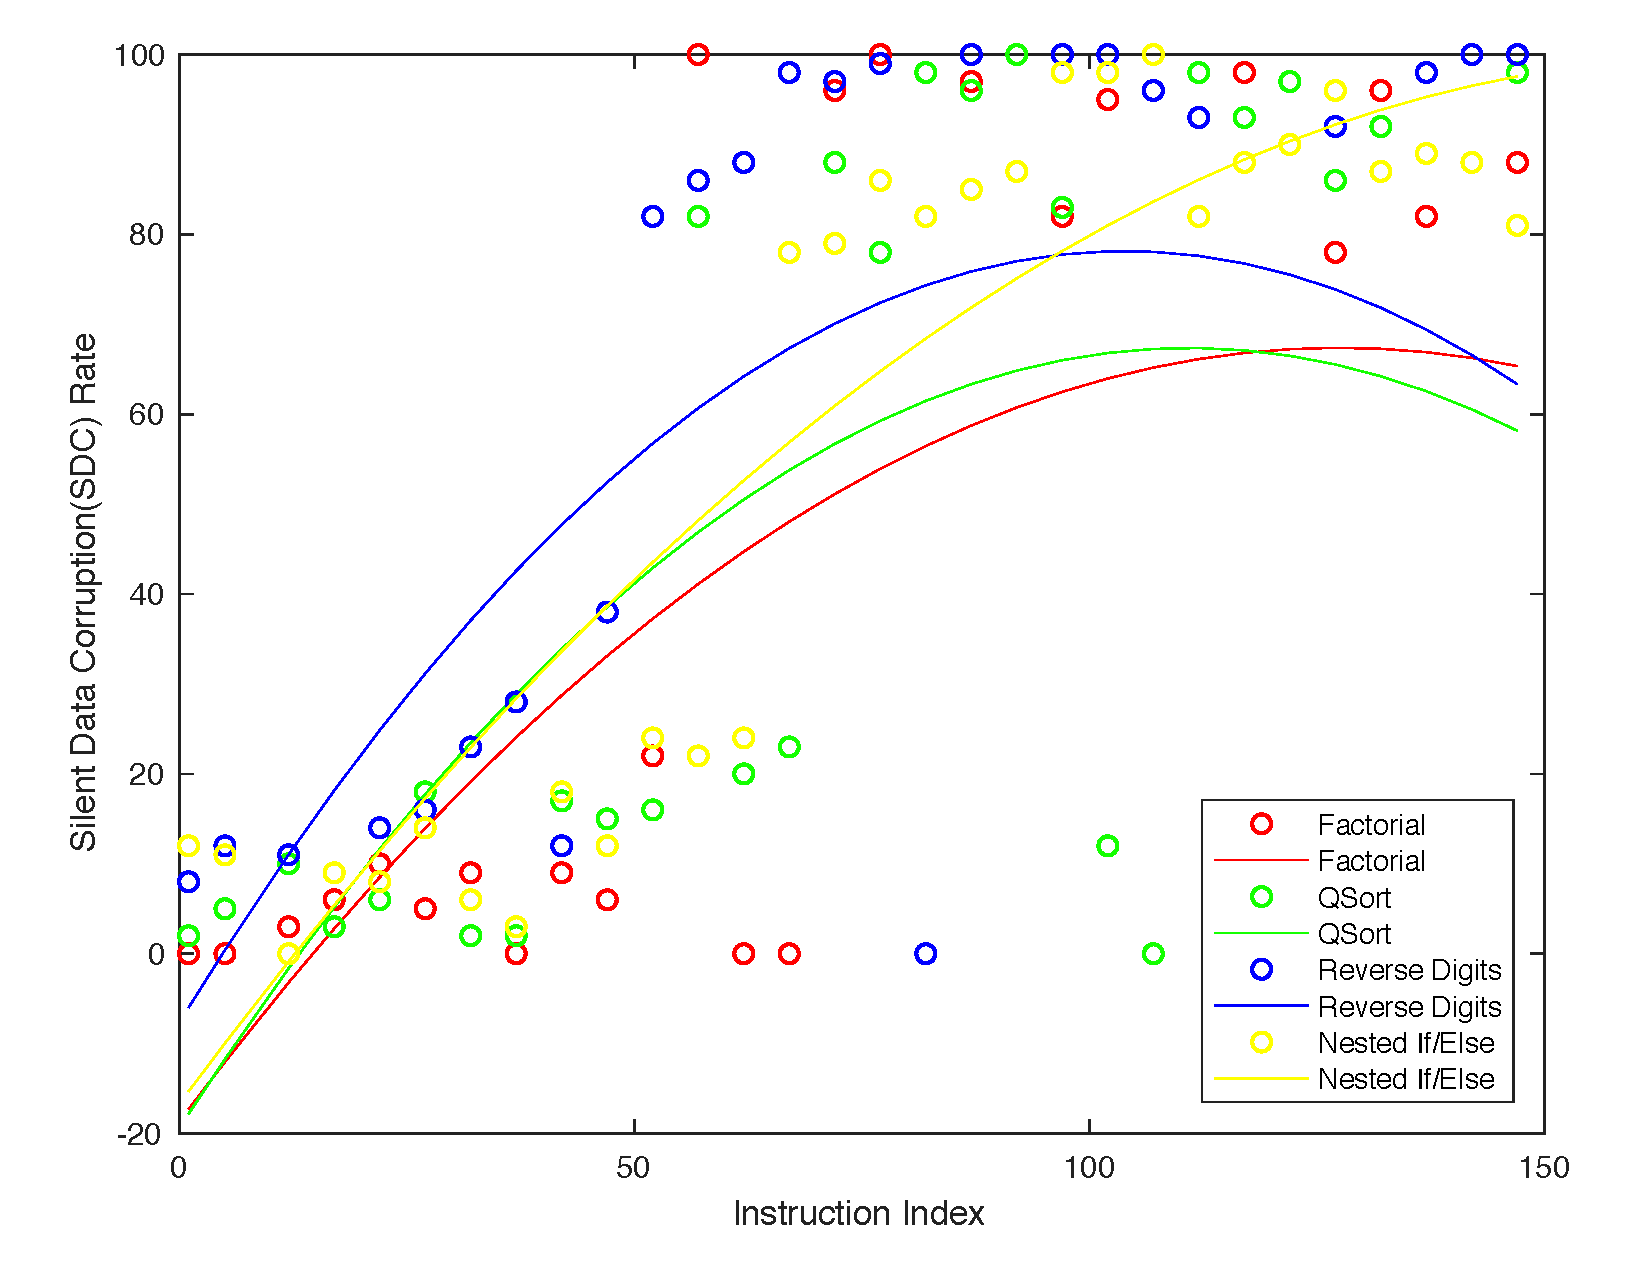
\includegraphics[scale=0.3]{./figures/figure_2_22.eps}
\end{center}
\caption{Relationship between the instruction index in control flow and its Silent Data Corruption percentage for different applications (Factorial, QSort, Reverse Digits, Nested If/Else).}
\label{fig:plan_8}
\end{figure}

\begin{figure}[!t]
\begin{center}
\label{fig:plan_5}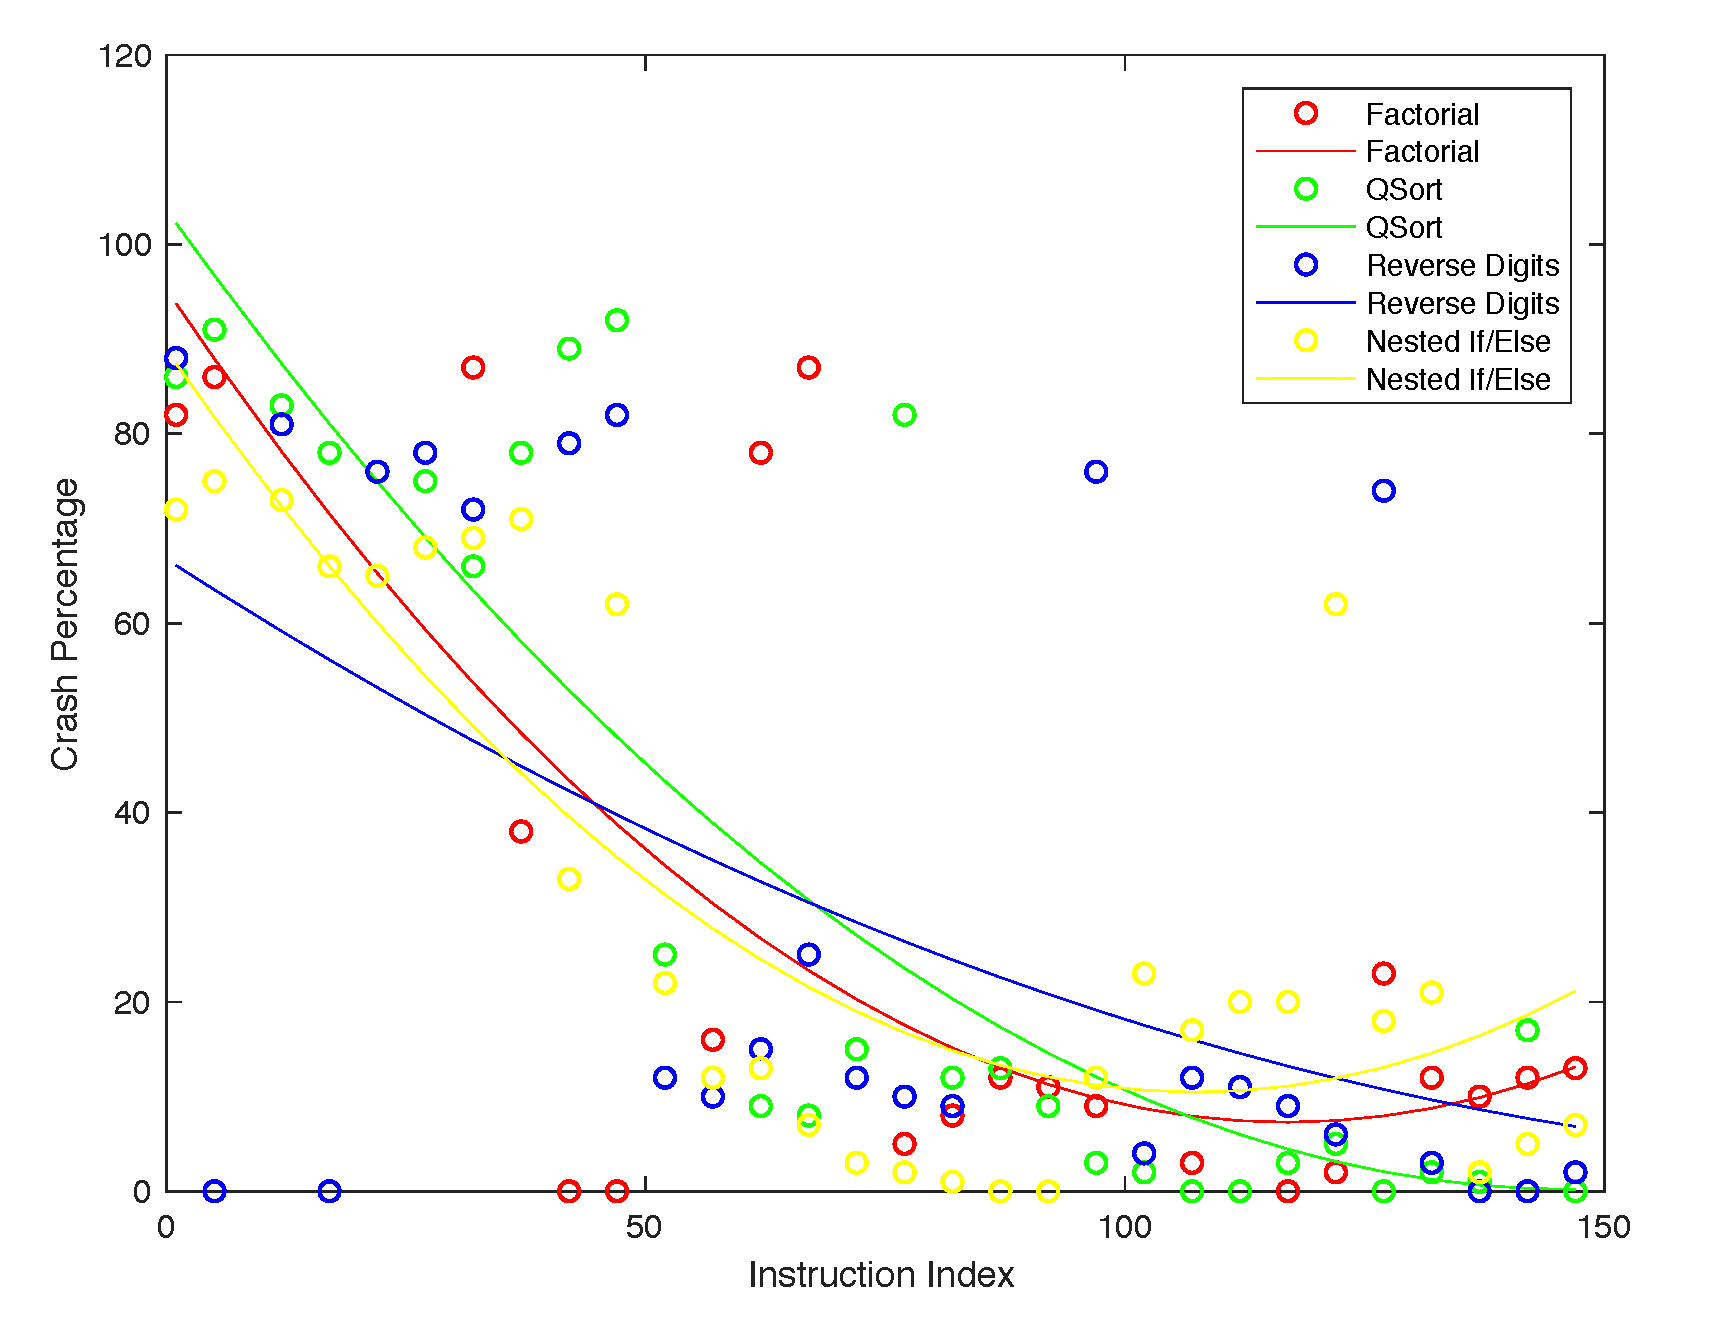
\includegraphics[scale=0.3]{./figures/figure_3_33.eps}
\end{center}
\caption{Relationship between the instruction index in control flow and its Crash rates for different applications (Factorial, QSort, Reverse Digits, Nested If/Else).}
\label{fig:plan_5}
\end{figure}

\begin{figure}[!t]
\begin{center}
\label{fig:plan_9}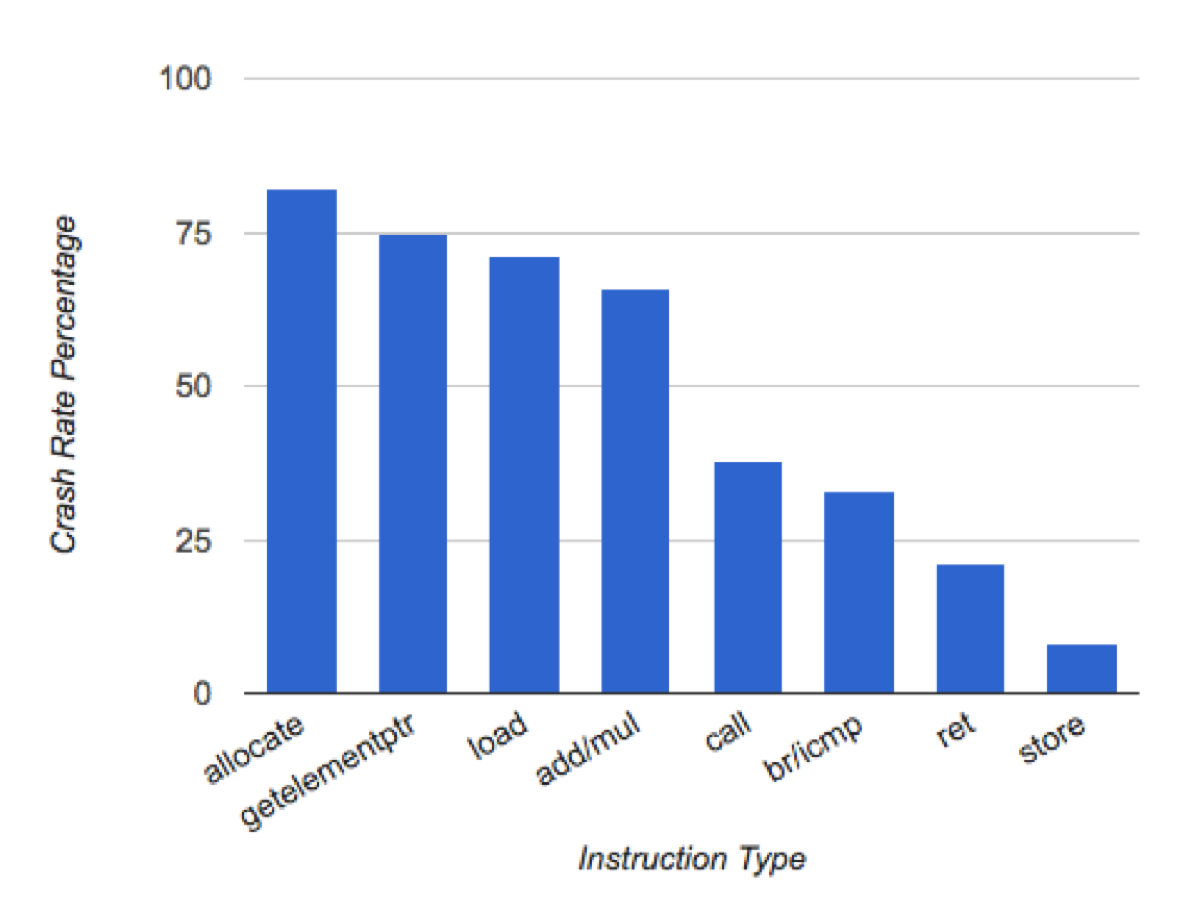
\includegraphics[scale=0.39]{./figures/crash_type_2.eps}
\end{center}
\caption{Crash rates for the most critical instructions. Rates are given as a percentage of their effect in the result.}
\label{fig:plan_9}
\end{figure}

\begin{figure}[!t]
\begin{center}
\label{fig:plan_10}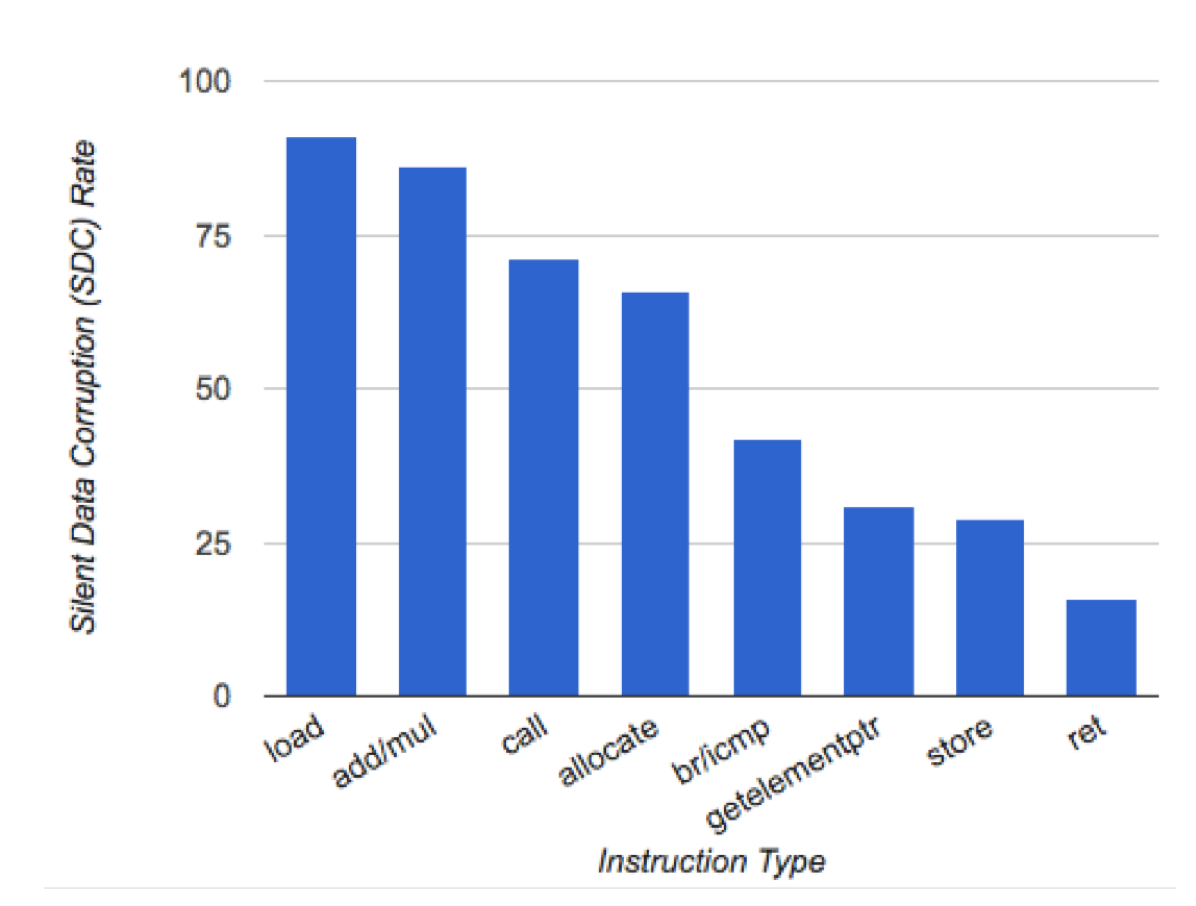
\includegraphics[scale=0.39]{./figures/sdc_type_2.eps}
\end{center}
\caption{SDC rates for the most critical instructions. Rates are given as a percentage of their effect in the result.}
\label{fig:plan_10}
\end{figure}



\subsection{Instruction Criticality}\label{sec:est_sharing}
% Discuss SDC and Crash results from previous subsection
% Explain the need for linear SDC and 1/Crash 
% Define the SDC and Crash metric with graphs
% Specify the importance of instruction location in control flow as percentage with small increments 
% Introduce the variable alpha as user input in detail 
% Discuss criticality due to repeated usage 
% Discuss the Data Dependency Constant*
% Normalization of values


In order to design a strong and widely applicable instruction ranking that would work for any source code with any amount of data, fault-injection tests are critical. The rates of SDC and Crash and their location in the control flow exhibit certain patterns. Since we observed that Silent Data Corruption rates are much higher in the final instructions of a program, there must be a direct relation between Silent Data Corruption and instruction location in the control flow. On the other hand, crash rates are much higher in the first basic blocks of CFG, which indicates an inversely proportional relationship between instruction location and Crash rates, as seen in Figures 2 and 3. 

Furthermore, our fault-injection experiments also showed that specific instruction types are less effective in Silent Data Corruption or Crash of a program. By observing average SDC and Crash values of each instruction type in various applications, we sorted the different instruction types separately for Silent Data Corruption and Crash of a program. Hence, we define two seperate reliability metrics for Silent Data Corruption and Crash.

The motivation behind these metrics is shown in Figures 4 and 5. These figures show significant results regarding the role of instruction type in our instruction criticality formula. As can be seen from these figures, some instruction types tend to crash or corrupt data significantly more than others. This, in turn, affects the corresponding instructions's vulnerability. Our fault injection results show that \emph{allocate} or \emph{load} operations are significant for both SDC and Crash. Moreover, since computations can affect the rate of Silent Data Corruption, it is observed that \emph{add} or \emph{mul} instructions are not SDC tolerant. By using the results based on instruction types, we ranked the instructions as shown in Table 1. Note that, for any other instruction that is not listed, the least-tolerant instruction value is used when calculating the instruction criticality of a specific instruction. While instruction types given in Table 1 are LLVM IR specific, our approach can easily be adopted to any low-level source code. More specifically, similar error injections can be applied to obtain instruction type ranking specific to the underlying architecture or instruction set. As can be seen from this table, most of these instructions are commonly found in any instruction set. Therefore, altough we use an LLVM specific setup, our approach is applicable to any architecture.

\begin{table}
\begin{center}
\caption
{
Individual instruction type rankings are presented where the first instruction type is the most significant type for Silent Data Corruption (or crash). The ranking values next to the instruction types should be considered for computing the instruction criticality. Instruction types that are not listed are treated as the least significant ranking. 
} 
\begin{tabular}{ p{2.5cm} p{2.5cm}}
 \textbf{Crash Rank}& \textbf{SDC Rank} \\
 \hline
 1. \emph{allocate} & 8. \emph{load} \\
 2. \emph{getelementptr} & 7. \emph{add/mul}  \\
 3. \emph{load} & 6. \emph{call}  \\
 4. \emph{add/mul} & 5. \emph{allocate}  \\
 5. \emph{call} & 4. \emph{br/icmp}  \\
 6. \emph{br/icmp} & 3. \emph{getelementptr}  \\
 7. \emph{ret} & 2. \emph{store} \\
 8. \emph{store} & 1. \emph{ret}  \\
\end{tabular}
\end{center}
\end{table}

Based on the SDC/Crash values with instruction location, we can use the rankings defined in Table 1 to create the first part of our instruction criticality formula. We define two variables, namely SDCm and Cm, where SDCm index has the value of the current instruction type from the SDC metric and Cm index has the value of the current instruction type in control flow from Crash metric, respectively. Finally, we define the variable $ILCF$ to represent the instruction location in the control flow in a normalized form. Specifically, $ILCF$ (Instruction Location in the Control FLow) can be calculated by dividing the index of the current instruction to the total number of instructions in the program.  We capture these properties in our instruction criticality (IC) formulation as follows:  
\begin{equation}
IC = (SDCm \times ILCF) + (\frac{1}{Cm \times ILCF}).
\end{equation}

The formula above calculates the criticality of any instruction in any source code. By looking at the instruction type of the current instruction from the metrics defined above and by calculating the right instruction location, we capture both SDC and Crash significance of an instruction. Note that the SDC and Crash rankings defined in Table 1 are created solely from the fault injection experiments on LLFI. It is important to state that these metrics could actually be parameterized, depending on the application. Since we conducted the fault injection experiments with a wide range of applications, we created our own rankings for SDC and Crash. We use these metrics to calculate the instruction criticality in our approach. However, depending on the application, there could be changes in the rankings of instruction types, which can be used for an application specific fault reduction technique. Our goal in this work is to create a common framework that can be used in any application.

As stated before, we introduce a variable $\alpha$ to the instruction criticality formula so that the user can decide whether the reliable source code should be more tolerant towards SDC or Crash. This variable will be an input to our approach and will be used in our formula to decrease or increase the criticality of SDC or Crash values. 

In addition to these, there are other factors that directly affect instruction criticality. While SDC or Crash of a program is highly significant for reliability, repeated usage of a single instruction will increase its potential damage. If an instruction is repeated constantly in a program (such as in a loop), probability of a soft error happening on that instruction would be higher. If a bit is flipped in such an instruction, the repeated use of that damaged instruction may produce catastrophic results. Based on this observation, we take loop index or loop count of an instruction into consideration where this loop count can be obtained from the compiler or a profiler. 

Furthermore, although the value of SDC captures the level of data dependency of a program to a certain extent, other factors for data dependency must also be considered. In order to better estimate the effects of data dependency, we define Data Dependency Constant (DDC) in our instruction criticality expression. Based on our experiments, we observe that bottom-up dataflow analysis fail to include major data dependency effects. Specifically, only a few instruction types are critically affected with huge amounts of data. Therefore, we use the DDC multiplier to increase the criticality of memory instructions (such as \emph{allocate}, \emph{load}, or \emph{store}). We apply DDC only to memory instructions since the data processing of a program are mainly dependent on these instructions. This way, our instruction criticality formula also considers data dependency of a given program.

Finally, based on the minimum and maximum values of each set of terms in our instruction criticality expression, we normalize the values to better reflect their impact. Our overall IC rank calculation is done according to the below formulation:
\begin{equation}
IC =(\alpha)(SDCm \times ILCF) + (1-\alpha)(\frac{1}{Cm \times ILCF})
+DDC+Loop Count 
\end{equation}

 In the above expression, LoopCount indicates the number of iterations a specific instruction gets executed as part of a loop (in case of a single execution this term is assumed to be 0). Our algorithm to calculate this IC metric and respective reliable source code generation will be presented in the next subsection. 



\subsection{Reliable Code Generation}

Reliable code generation depends on the instruction criticality formula we presented. By using the instruction criticality and the input source code, we apply the formula to each instruction in the code. First, we parse the IR file using built-in LLVM \cite{LLVM:2004} libraries and generate an instruction index for each instruction. We save each instruction's index and the instruction type which then is used with SDC metric and Crash metric to calculate instruction's criticality. Then, we sort these instructions based on their criticality value. After this point, we have the most critical instructions sorted which we modify the source code based on the given overhead limit. This overhead tolerance limit is considered as the percentage increase in execution cycles.

Specifically, we apply one of the state-of-the-art reliability techniques to the most critical number of instructions in such a way that the overhead limit will be met. After applying these, we generate reliable source code with minimal overhead. The algorithm to achieve this code generation is presented in Algorithm 1. Note that the input variable overhead in the algorithm is to be captured dynamically depending on the dynamic execution time of the program. It is fair to state at this point that ignoring least-critical instructions when applying reliability improvements increases performance and reduces other potential overheads.

 As stated before, the reliability technique to be used in this setup is orthogonal to our approach. Even though we used  EDDI (Error Detection by Duplicating Instructions) \cite{EDDI:2002} for experimental results, any other source code reliability technique could be used. Since the aim of this paper is to capture the importance of instruction criticality and reduce the total overhead, different reliability techniques can potentially make use of our approach.

\begin{algorithm}
\SetKwData{Left}{left}\SetKwData{This}{this}\SetKwData{Up}{up}
\SetKwFunction{Union}{Union}\SetKwFunction{FindCompress}{FindCompress}
\SetKwInOut{Input}{inputs}\SetKwInOut{Output}{output}
\Input{IR\_file, $\alpha$, Overhead}
\Output{Reliable Source Code}
\BlankLine
$Instruction\_Types[] \longleftarrow ParseIRFile(IR\_file)$ \\
$size \longleftarrow size(Instruction\_Types)$ \\

\For{$i\leftarrow 0$ \KwTo $size$}
{
\For{$j\leftarrow 0$ \KwTo $8$}
{
\If{$SDCm[j] = Instruction\_Types[i]$}
{
$current\_SDC \longleftarrow SDCm[i]$
}
\If{$Cm[j] = Instruction\_Types[i]$}
{
$current\_Crash \longleftarrow Cm[i]$
}
}
$ILCF \longleftarrow i / size$\\
\If{$Instruction\_Types[i]='allocate' || 'load' || 'store'$}
{
  $DDC \longleftarrow 0.55$
}
\Else{$DDC \longleftarrow 0$}
$IC\_Array[i][Instruction\_Types[i]] \longleftarrow alpha * current\_SDC * ILCF + (1-alpha)(1/(current\_Crash * ILCF) + DDC + LLVM.LoopCount$
}
MergeSort($IC\_Array$)\\
$index \longleftarrow 0$ \\
\While{$dynamic\_execution \leq Overhead$}
{
   $ReliableCode$ $\longleftarrow$ Apply\_Technique($index, IR\_file$)\\
   $index \longleftarrow index + 1 $ \\
}
\textbf{return} $ReliableCode$
\caption{Our algorithm to generate reliable source code based on our instruction criticality formula.}
\end{algorithm}

\section{Experimental Evaluation}\label{sec:evaluation}

\subsection{Setup}
We tested our reliable code generation algorithm on different benchmarks from Media Bench \cite{MediaBench:1997} and MiBench \cite{MiBench:2001}. The set of benchmark codes used in our experiments are given in Table 2. The third column of this table explains the functionality implemented by each benchmark. The next two columns give the number of basic blocks and code size in kilobytes, respectively. The last column gives the dynamic nymber of instructions executed. 

We collected statistics for a number of different applications in each benchmark and compared the SDC and Crash rates with non-modified source codes. After implementing our code generation algorithm, we again used LLFI \cite{LLFI:2015} on different benchmark applications where we first injected faults in a random manner without any modification. Then, for different overhead limits and different $\alpha$ values, we injected faults similarly to our proposed approach. In order to get accurate results, at least a thousand fault injections were conducted on the source code using a random number generator. All experiments are repeated multiple times and the average values of those experiments were reported. 

For each benchmark code in our experimental suite, we performed experiments with 3 different versions, which can be summarized as follows.\\
1)\emph{BASE}: The base execution does not employ any optimization where we injected randomized faults into unmodified LLVM IR code and collected data. \\
2)\emph{ICBR}: This is our instruction criticality based reliability (ICBR) enhancement approach where we applied our reliable code generation algorithm and collected both SDC and Crash results. \\
3)\emph{FTP}: Finally, we conducted fault injection experiments on fully tolerant and protected (FTP) programs so that we could see how close we are to a fully fault-tolerant system with a given $\alpha$ and overhead.\\

Finally, Table 3 lists the base simulation parameters used in our experiments. Unless stated otherwise, our results are collected using these parameters. We use $\alpha$ as 0.5 for the default value since we want to keep the significance of SDC and Crash the same. Note that this value can easily be changed by the user. We also set the overhead limit as 70\% to compare and prove the usefulness of our formula. Finally, we use 0.55 as the default value for DDC after our analysis and normalization of our IC formula. 


\begin{table}
\begin{center}
\caption{Benchmarks used in our experiments and their characteristics.} 
\begin{tabular}{ p{1.2cm} p{2.2cm} p{2.2cm} p{1cm} p{0.5cm} p{0.6cm} }
 Benchmark& Source & Type & Number of Basic Blocks& Code Size (KB)& Instr Count (mil)\\
 \hline
 btcnt& MiBench \cite{MiBench:2001} & Automative &  138 &  98 &  688.3 \\
 btstrng& MiBench \cite{MiBench:2001} & Automative&  56 &  48.9 &  327.3 \\
 FFT& MiBench \cite{MiBench:2001} & Telecomm & 44 & 69.2 & 238.89 \\
 qsort& MiBench \cite{MiBench:2001} & Automative & 78 &  72.3 &  513.8 \\
 adpcm& MediaBench \cite{MediaBench:1997} & Compression & 22 & 8 & 1.2\\
 gsm& MediaBench \cite{MediaBench:1997} & Telecomm & 98  &  438   &  7.09  \\
 jpeg& MediaBench \cite{MediaBench:1997} & Decompression &  112  &  488.8  &  18.65  \\
 rasta& MediaBench \cite{MediaBench:1997} & Feature Extraction &  189  &   269  &  24.86   \\
\end{tabular}
\end{center}
\end{table}


%%% TABLE HERE FOR BASELINE PARAMETERS %%%% 
\begin{table}
\begin{center}
\caption
{
Baseline parameters used in our experiments.
} 
\begin{tabular}{ p{2.5cm} p{2.5cm} }
 \textbf{Parameter}& \textbf{Default Value} \\
 \hline
 $\alpha$ & 0.50 \\
 Overhead limit & 70\% \\
 DDC & 0.55 \\
\end{tabular}
\end{center}
\end{table}

\begin{figure}[!t]
\begin{center}
{\label{fig:plan_11}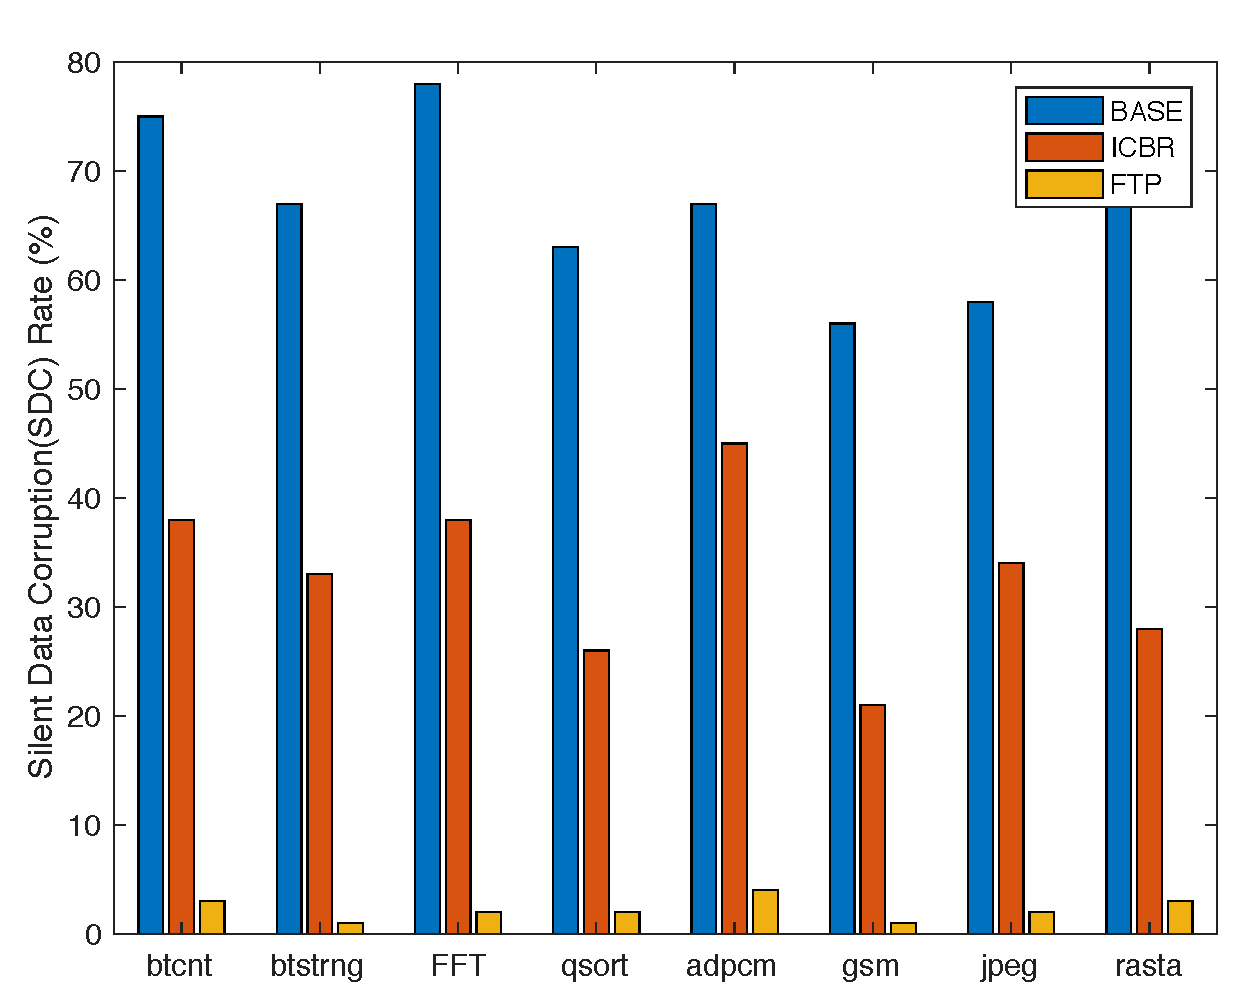
\includegraphics[scale=0.4]{./figures/Figure_9_final.eps}}
\end{center}
\caption{Fault injection results for BASE, ICBR and FTP for our benchmarks.}
\label{fig:plan_11}
\end{figure}

\begin{figure}[!t]
\begin{center}
{\label{fig:plan_12}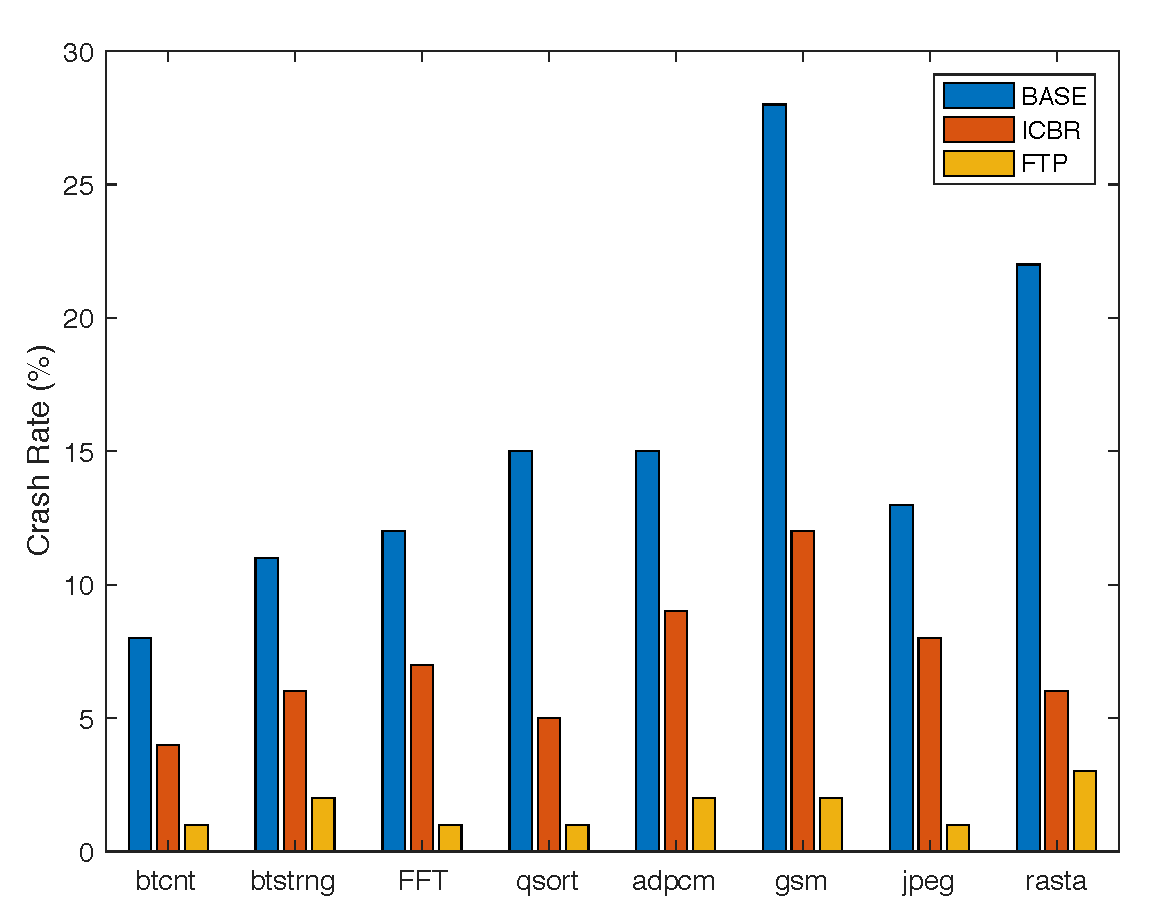
\includegraphics[scale=0.42]{./figures/Figure_10_ff.eps}}
\end{center}
\caption{Fault injection results for BASE, ICBR and FTP for our benchmarks.}
\label{fig:plan_12}
\end{figure}

\begin{figure}[!t]
\begin{center}
{\label{fig:plan_13}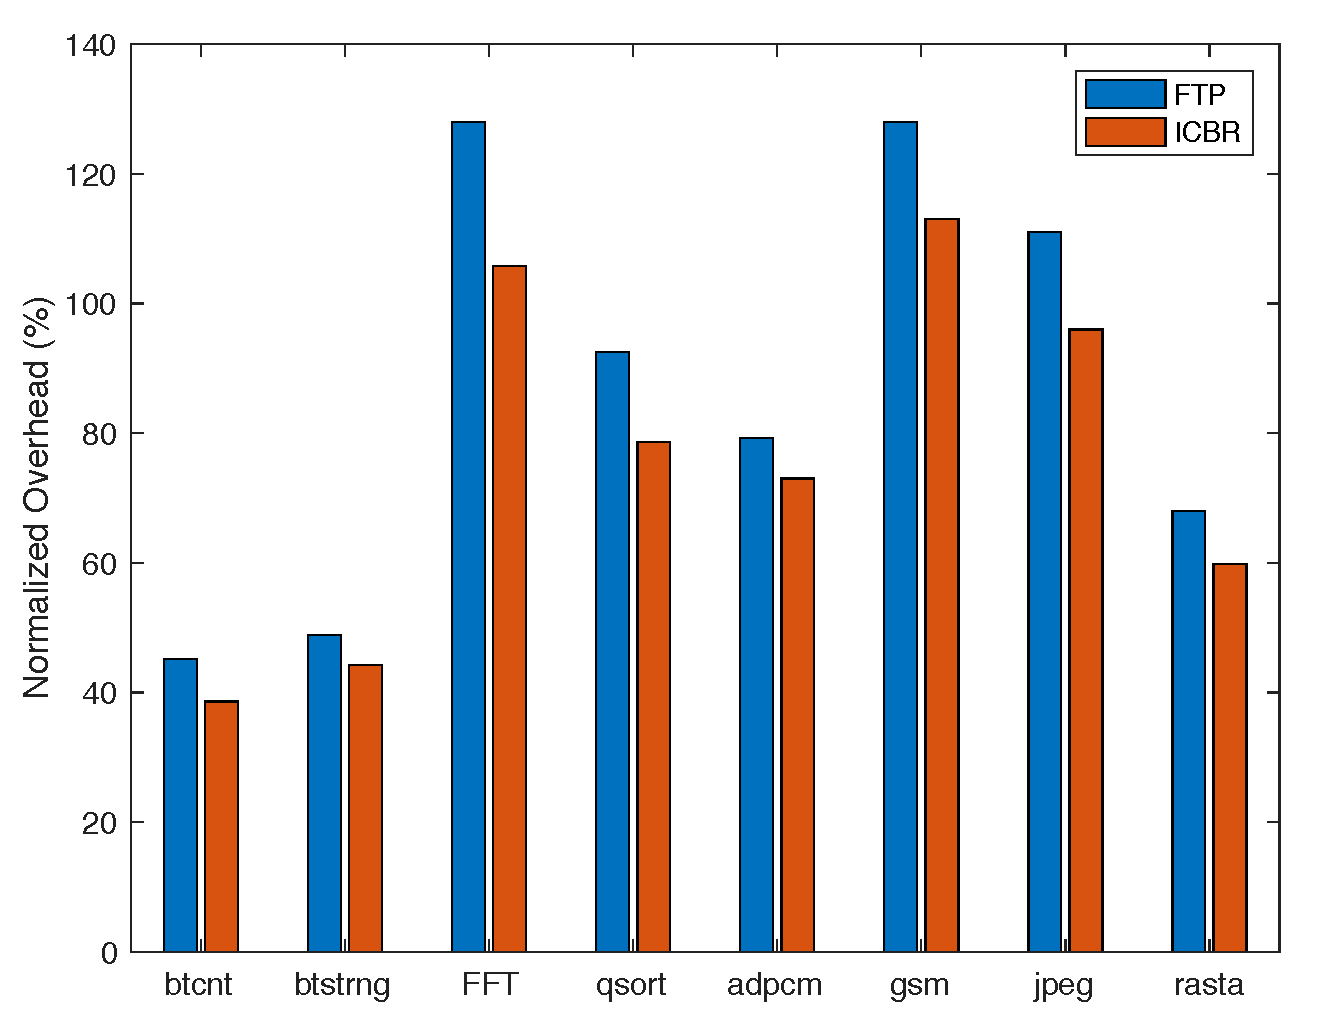
\includegraphics[scale=0.42]{./figures/baseline_overhead.eps}}
\end{center}
\caption{Performance overhead in FTP and ICBR normalized with respect to BASE.}
\label{fig:plan_13}
\end{figure}



\subsection{Results}\label{sec:Results}
Experimental results presented in this paper are based on two inputs to our approach; $\alpha$ and the overhead limit. As stated before, based on these inputs, we collected results on 3 different versions of each source code; BASE, ICBR, and FTP. It is significant to state that both MiBench and MediaBench produced similar results. 

Our first set of results describe the fault injections on our benchmarks BASE, ICBR and FTP  to analyze the SDC rate. Based on analysis with our criticality formula, we set $\alpha$ to 0.5 and the overhead limit to 70\%. As stated before, these parameters are chosen this way to compare our approach with different versions in a detailed way. As can be seen from Figure 6, data corruption rates decrease significantly with our approach compared to the BASE case. More specficically, our approach reduces SDC rate from 67\% to 32\% on average when compared with the BASE case. On the other hand, our results are higher when compared to the average SDC rate of 8\% for FTP. However, this is expected since our approach limits the performance overhead to 70\% by default, whereas FTP incurs 115\% of performance overhead on the average as a result of full protection. 

The next set of experiments show the effects of fault injections on Crash rates. As can be seen from Figure 7, BASE results with an average of 8\% to 28\% Crash rates, whereas this range is reduced to an average of 1\% to 5\% for FTP. Our approach, on the other hand, have Crash rates ranging from 4\% to 14\%. On the average, our approach reduces the Crash rates from 17\% to 8\% when compared to BASE. Similar to SDC, Crash rates are also higher with respect to FTP due to the performance overhead limitation enforced. 

Based on the results shown in Figure 6 and 7, one can observe that data corruption rates and crashes are reduced with a limited overhead.

%%%%%%% ADD FIGURE 8 ANALYSIS HERE!!!! %%%%%%%%%
In the next set of experiments, we present the performance overhead of FTP and ICBR results where the execution time is normalized with respect to BASE. As can be seen in Figure 8, the two overhead results are similar where ICBR has shorter execution time compared to FTP. More specifically, FTP results indicate an average of 101\% overhead with respect to BASE whereas ICBR data indicate an average of 83\% overhead with respect to BASE. 


\subsection{Sensitivity Analysis}\label{sec:Sensitivity}
As explained before, $\alpha$ is used to specify the significance of the data corruption or Crash tolerance in an application. Hence, we change $\alpha$ for each source code and analyze the sensitivity of the variable in the error rates. The $\alpha$ parameter is significant for our results since in some applications the Crash rates are considerably low. 

\begin{figure}[!t]
\begin{center}
{\label{fig:plan_13}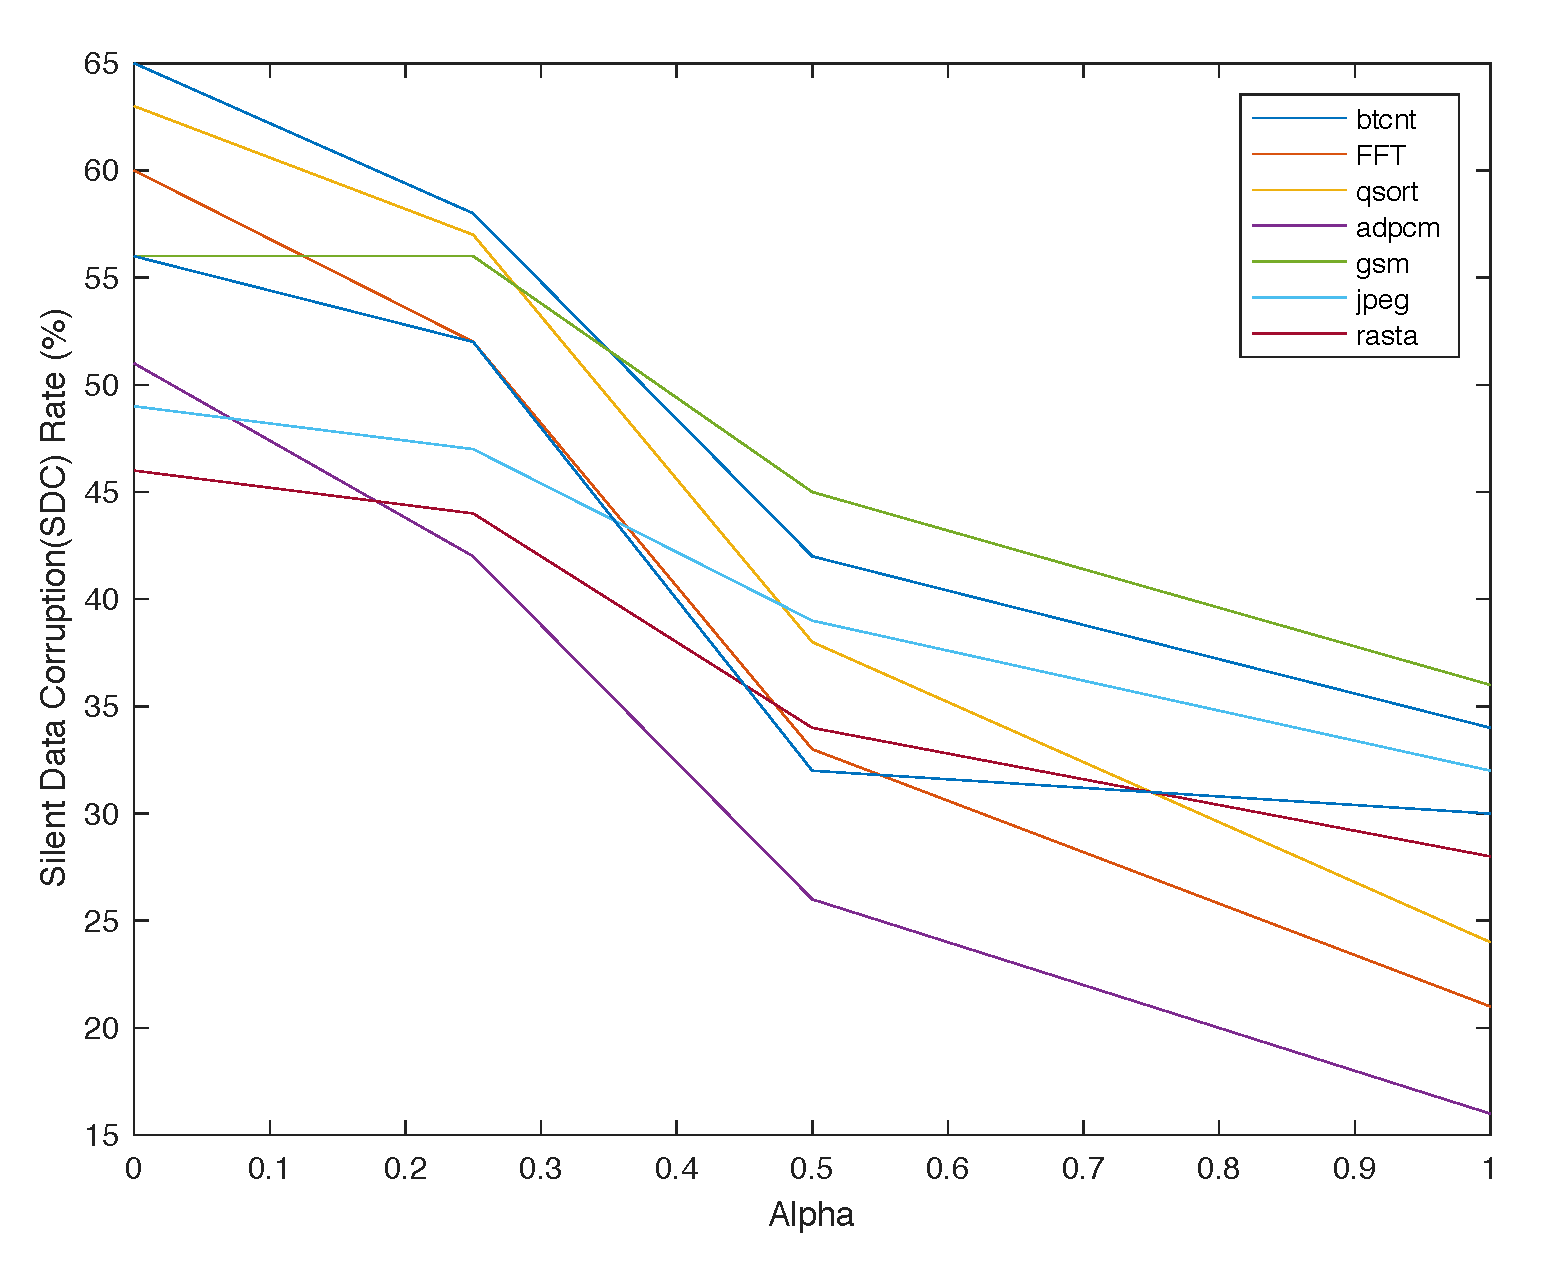
\includegraphics[scale=0.32]{./figures/figure9.eps}}
\end{center}
\caption{Sensitivity of Silent Data Corruption (SDC) on $\alpha$ for our benchmarks.}
\label{fig:plan_13}
\end{figure}

\begin{figure}[!t]
\begin{center}
{\label{fig:plan_14}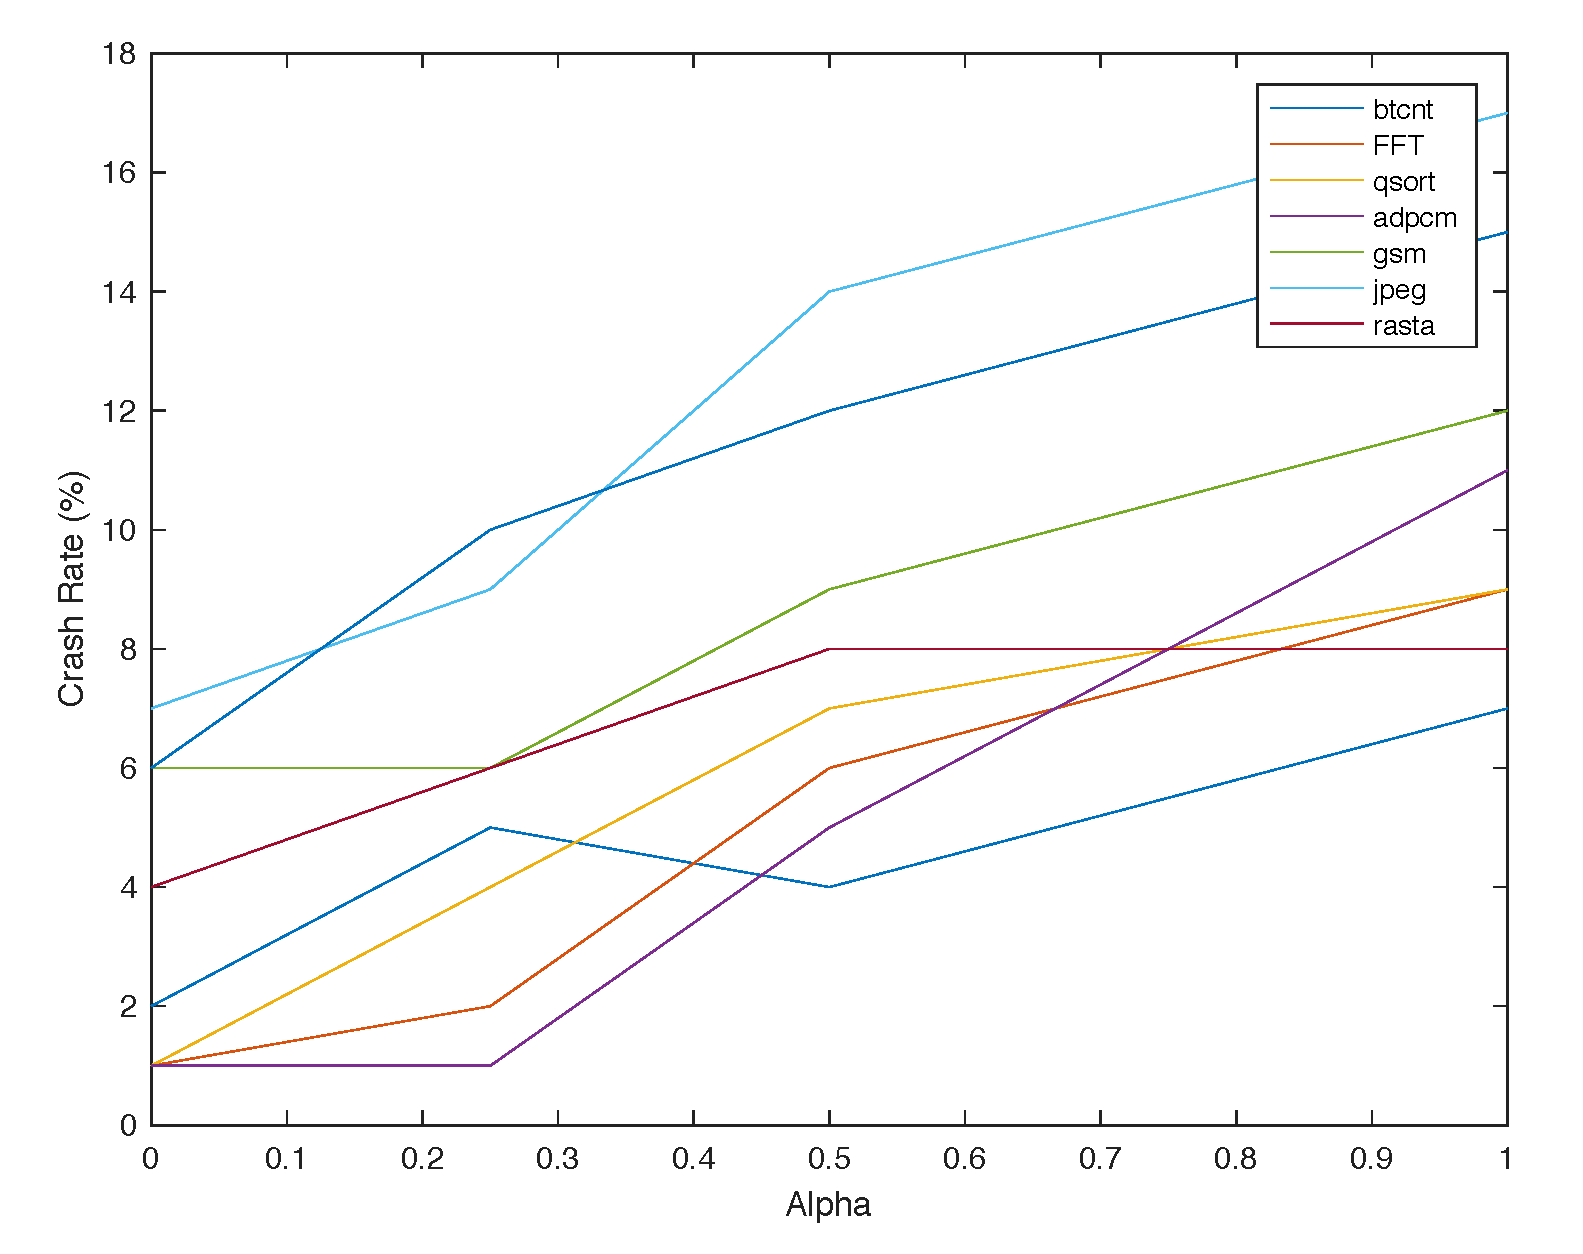
\includegraphics[scale=0.32]{./figures/figure10.eps}}
\end{center}
\caption{Sensitivity of Crash on $\alpha$ for our benchmarks.}
\label{fig:plan_14}
\end{figure}

\begin{figure}[!t]
\begin{center}
{\label{fig:plan_15}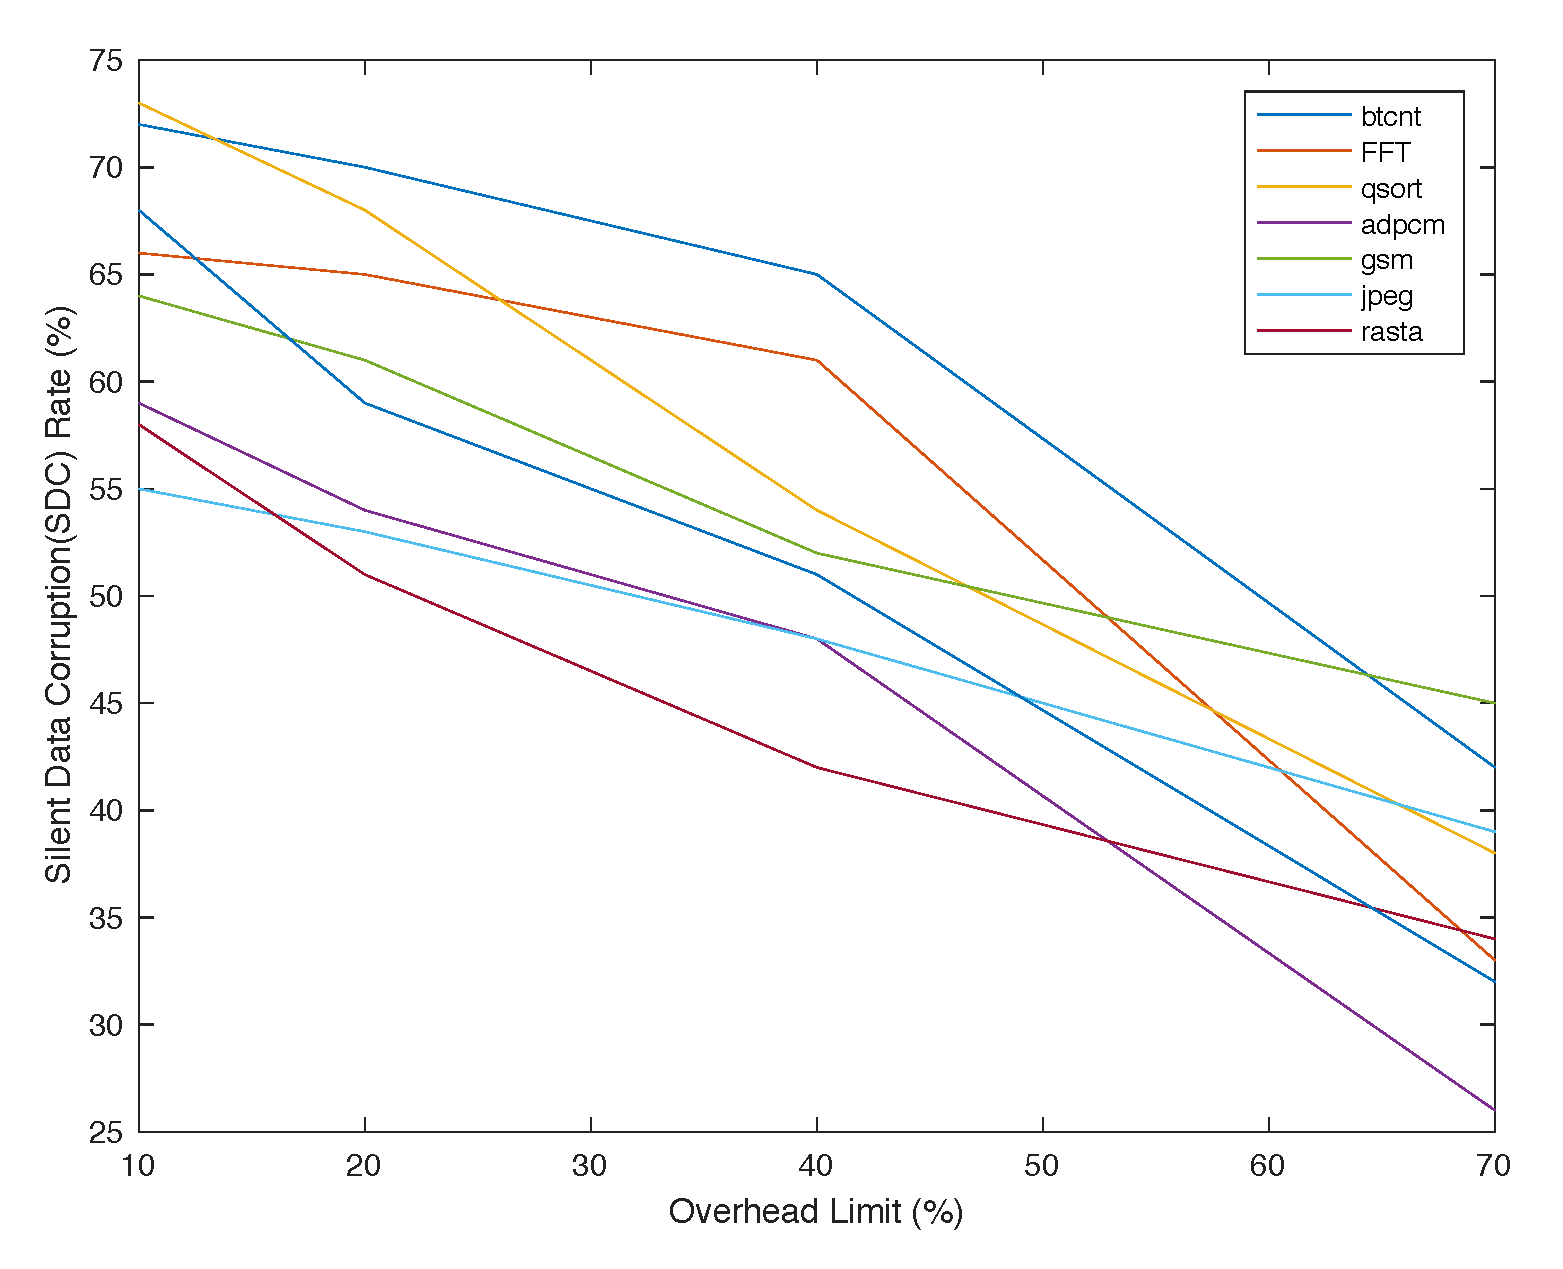
\includegraphics[scale=0.32]{./figures/figure11.eps}}
\end{center}
\caption{Sensitivity of Silent Data Corruption (SDC) on overhead limit for our benchmarks.}
\label{fig:plan_15}
\end{figure}

\begin{figure}[!t]
\begin{center}
{\label{fig:plan_16}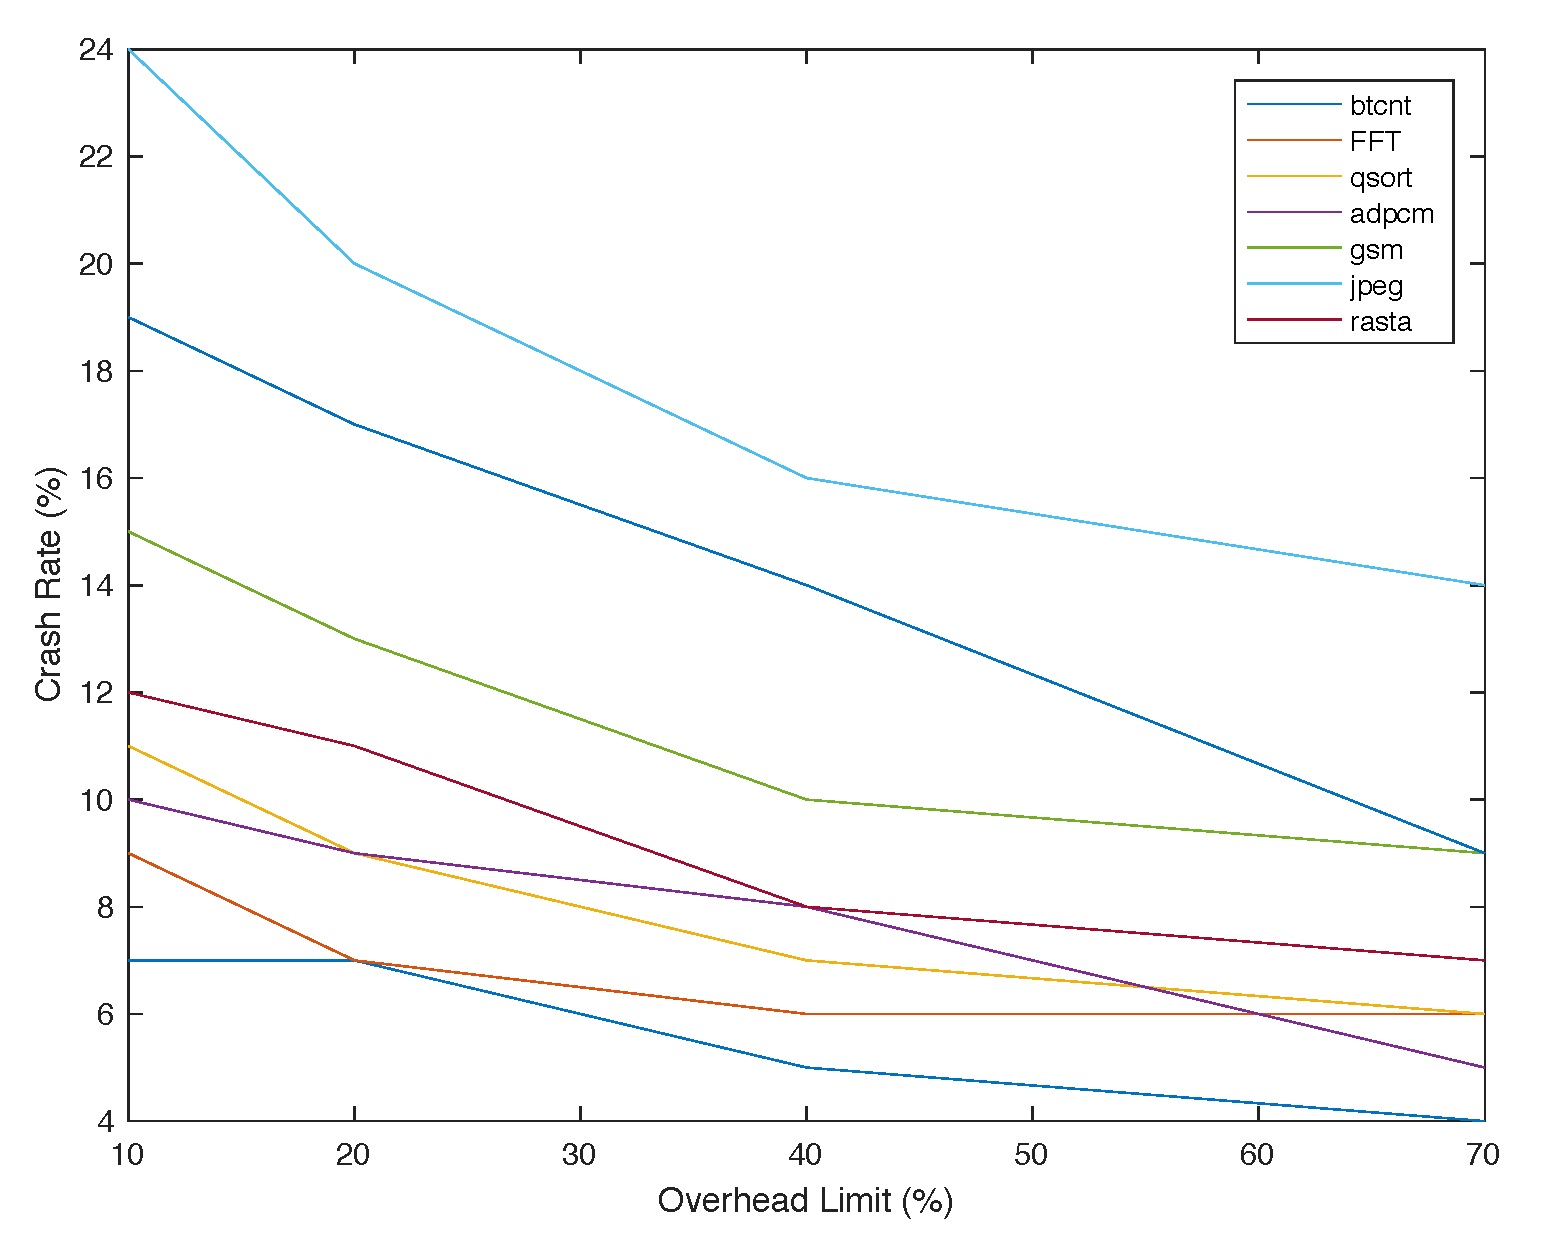
\includegraphics[scale=0.32]{./figures/figure12.eps}}
\end{center}
\caption{Sensitivity of Crash on overhead limit for our benchmarks.}
\label{fig:plan_16}
\end{figure}



Figures 9 and 10 shows the SDC and Crash rates with increasing $\alpha$ values for our benchmarks. We kept the overhead limit constant at 70\% to only focus on the effect of $\alpha$ in our approach. Starting from 0, we increased $\alpha$ until 1 with 0.25 increments. As seen from Figure 9, the rate of SDC decreases for each benchmark with increasing $\alpha$. This is because higher $\alpha$ values increase the significance of SDC in our instruction criticality formula. On the other hand, Figure 10 shows that Crash rates increase with increasing $\alpha$. As expected, lower $\alpha$ increases the focus on Crash tolerance.  


In the next set of experiments, we increase the overhead limit based on the dynamic execution of the application and keep a consistent rate of change each time. Specifically, we change the dynamic overhead limit with respect to total execution time of the BASE and conduct fault injection experiments on the benchmarks. Figures 11 and 12 show the SDC and Crash rates with increasing overhead limit ranging from 10\%, to 70\%. As can be seen from figures, both SDC and Crash rates tend to decrease with increasing overhead. A decrease of 10\% in SDC and 5\% in Crash rates is possible with only 20\% dynamic overhead limit. On the other hand, when the overhead limit is increased to 70\%, there was at least a 35\% decrease in SDC rate and a 10\% decrease in Crash rate. Crash rate tend to decrease slower since BASE has low crash rates in the beginning. 


\section{Conclusion}\label{sec:conclusion} 

In this paper, we attempt to decrease the overhead caused by state of the art reliability techniques by presenting an instruction criticality formula and a reliable code generation algorithm. We show that instruction criticality is heavily dependent on instruction type, instruction location in control flow and execution frequency. Taking these into consideration, we present our approach on reliable code generation where current reliability techniques are applied only to most critical instructions.  Our LLVM-based implementation provides encouraging results in our experiments on MiBench and MediaBench. We observe 35\% decrease in Silent Data Corruption (SDC) rate and a 10\% decrease in Crash rate on average when we limit the performance by 70\%. It is also important to note that, even with a small overhead as low as 10\%, we are able to increase fault tolerance up to 8\%. 
